This Software Requirements Specification (SRS) outlines the software and system requirements for Rahguzar, a route optimization project aimed at improving efficiency in retail and distribution. It details functional requirements for system capabilities and non-functional requirements like performance and scalability. The document also includes system block diagrams, use cases, and external interfaces to clarify the system’s design and interactions.

\section{Functional Requirements}


% This section describes each function/feature provided by our system. These functions are logically grouped into modules based on their purpose/users/mode of operations etc (as per our system). A functional hierarchy may look like:
% \begin{outline}
%   \1 Module 1:
%   \2 Function 1:
%   \2 Function 2:
%   \3 Sub Function 1
%   \3 Sub Function 2
%   \1 Module 2:
%   \2 Function 1:
%   \2 Function 2:
%   \1 .........
% \end{outline}




The functional requirements for this system focus on creating an efficient journey-planning solution tailored for order bookers and sales representatives. This system is designed to optimize routes based on key operational parameters and provide dynamic rerouting, while also supporting targeted store visits and frequency schedules. Additional modules include a user-friendly web platform, pilot testing and validation, and performance monitoring to ensure enhanced efficiency and measurable sales impact.The following are the functional requirements for each module and their respective functions.

\subsection*{Module 1: Route Optimization Algorithm}
\subsubsection*{Function 1: Route Generation}
\begin{itemize}
    \item Implement an algorithm that creates journey plans optimized for order bookers and sales representatives.
    \item The optimization should consider multiple factors:
    \begin{itemize}
        \item[] \textbf{Sub Function 1: Order Booker Shift Times} \\
            Align route planning with the working hours of each order booker.
        \item[] \textbf{Sub Function 2: Number of Shops to Visit} \\
            Adjust routes to maximize the number of shops visited within constraints.
        \item[] \textbf{Sub Function 3: Number of Order Bookers Available} \\
            Allocate routes based on the number of available staff.
        \item[] \textbf{Sub Function 4: Total Distance Traveled} \\
            Minimize the total distance covered during journeys.
        \item[] \textbf{Sub Function 5: Total Travel Time} \\
            Reduce the time taken to complete the planned routes.
        \item[] \textbf{Sub Function 6: Store Service Times} \\
            Account for different service time requirements at each store.
    \end{itemize}
\end{itemize}
 \begin{itemize}
     \item Include a feature to assign priority to specific parameters to adapt the optimization to business needs.
 \end{itemize}

\subsubsection*{Function 2: Dynamic Rerouting}

    % \item Integrate a feature to adjust routes based on updated data (e.g., traffic, store closure).
    % \item The rerouting should optimize new paths instantly to maintain efficiency.

    \begin{itemize}
        \item It allows users to interactively adjust key parameters of the route optimization algorithm, such as the number of order bookers and the number of stores per booker, directly on the display screen.
        \item It simply enables real-time rerouting, with the algorithm instantly updating the allocation of stores and route paths to reflect user preferences, providing flexibility and adaptability in journey planning.
    \end{itemize}

 

% \subsection*{Module 2: Weekly Store Visit Optimization 
% }

\subsubsection*{Function 3 : Store Visit Frequency: 
}

\begin{itemize}
    \item Design the algorithm to include visit frequency for each store (e.g., once, twice, or three times a week).
    \item Ensure that the routes align with required visit frequencies without any overlap or gaps.
\end{itemize}

\subsubsection*{Function 4: Journey Planning for Different Timeframes: 
}

\begin{itemize}
    \item Support the generation of routes 
by allowing monthly PJP creation with customizable weekly patterns (like odd/even weeks) and enable downloads for extended periods, such as a year. based on the target timeframe.
    \item Ensure that stores are scheduled accurately according to their frequency needs while minimizing travel and maximizing coverage.
\end{itemize}



 

% \subsection*{Module 3: Store Profile Management and Integration }

\subsubsection*{Function 5: Store Profiling: }

\begin{itemize}
    \item Maintain detailed profiles for each store, including:
    \begin{itemize}
        \item[] \textbf{Sub Function 1:} Geographical hierarchy (region, zone, territory, town).
        \item[] \textbf{Sub Function 2:} Sales channel type (e.g., wholesale or retail).
    \end{itemize}
    \item Enable users to filter stores by parameters like region, sales channel, or visit frequency. Allow custom filters linked to all stores by uploading relevant data (e.g., location, sales volume), enabling dynamic application across stores. This approach enhances flexibility and control in route optimization.
\end{itemize}

\subsubsection*{Function 6: Targeted Journey Plans:}
 
\begin{itemize}
    \item Enable the system to generate routes targeting specific store types (e.g., only wholesale stores in a particular region).
\end{itemize}

 

\subsection*{Module 2: Web Application Platform 
}

\subsubsection*{Function 1: User Interface for Route Management: 
}

\begin{itemize}
    \item Create a user-friendly web interface for managers to access and manage journey plans.
\end{itemize}
\subsubsection*{Function 2: Integrate Map Interface:
}

    \begin{itemize}
        \item Designing, viewing, and adjusting routes.
        \item Displaying essential shop details (e.g., store profiles, geographical location).
        \item Defining and viewing boundaries like regions, territories, and areas.
    \end{itemize}

\subsubsection*{Function 3: Manual Override and Adjustment: 
}

\begin{itemize}
    \item Provide a manual override feature that allows managers to create or adjust routes manually, even if automated suggestions exist.
    \item Include input options for master data (store profiles, visit frequencies, geographical details) directly within the platform.
\end{itemize}

\subsubsection*{Function 4: Downloadable Reports: 
}

\begin{itemize}
    \item Allow users to export optimized or manually adjusted routes in a downloadable format for offline analysis or distribution.
\end{itemize}

\subsection*{Module 3: Pilot Testing and Validation }

\subsubsection*{Function 1: Test Plan Creation: 
}

\begin{itemize}
    \item Develop a comprehensive pilot testing framework to validate the system's effectiveness.
\end{itemize}
\subsubsection*{Function 2: Real-World Data Integration: }

\begin{itemize}
    \item Gather real-world data during pilot testing, ensuring data is accurate and reliable.
\end{itemize}

\subsubsection*{Function 3: Performance Assessment: }
\begin{itemize}
    \item Collect and analyze data (travel time, number of shops visited, sales impact, etc.) to assess system performance.
    \item Implement an adjustment process based on pilot feedback to enhance the algorithm.
\end{itemize}

\subsubsection*{Function 4: Case Study Development: }

\begin{itemize}
    \item Compile a case study summarizing the outcomes, findings, and system performance.
\end{itemize}

\subsection*{Module 4: Performance Monitoring and Reporting }

\subsubsection*{Function 1: Key Performance Indicators (KPIs): }

\begin{itemize}
    \item Track and display metrics like:
\end{itemize}
    \begin{itemize}
    \item[] \textbf{Sub Function 1:} Average travel time per route.
    \item[] \textbf{Sub Function 2:} Number of shops visited per shift.
    \item[] \textbf{Sub Function 3:} Number of order bookers required per distribution.
    \item[] \textbf{Sub Function 4:} Sales uplift due to route optimization.
    \item[] \textbf{Sub Function 5:} Algorithm response time for route recalculations.
\end{itemize}
 

\subsubsection*{Function 2: North Star Metric Tracking: 
}

\begin{itemize}
    \item Focus on monitoring the primary metric: "Increase in average daily sales per sales representative."
\end{itemize}

\subsubsection*{Function 3: Metrics Dashboard:
}

\begin{itemize}
    \item Develop a dashboard to visualize KPIs, providing insights into efficiency improvements, time savings, and sales increases.
\end{itemize}









% --- The above is to be modified as per your project, e.g. a flat list if your system has limited functional requirements.

\section{Non-functional Requirements}

% This sections mentions the specific non-functional requirements of our system. These generally address performance, scalability, safety, availability, deployment etc.

The Non-functional requirements define the quality and performance attributes of this system, focusing on scalability, usability, and reliability. They ensure optimal performance under varying conditions while maintaining data security and adaptability for user needs. Additionally, following requirements also facilitate maintainability for future enhancements, ensuring the system remains effective over time.








\begin{enumerate}
    \item \textbf{Scalability, Efficiency, and Memory Optimization}
    \begin{itemize}
        \item The system is designed to efficiently handle large datasets and scale up to 2000 stores effectively as the amount of data increases, ensuring optimal performance and quick response times within 2 minutes for route generation.
        \item It should also have a low memory footprint, ensuring that it can scale effectively without degrading system performance or requiring excessive computational resources.
    \end{itemize}
    
    \item \textbf{Usability}
    \begin{itemize}
        \item A user-friendly web application interface is required, allowing users to manage, optimize, and adjust journey plans easily.
        \item The map interface must provide intuitive visualization and interactivity for planning and real-time adjustments.
    \end{itemize}
    \newpage
    \item \textbf{Reliability and Performance}
    \begin{itemize}
        \item The AI-driven route optimization algorithm should be robust, quickly generating optimal routes based on parameter changes, such as order booker shifts or the number of stores per booker.
        \item The system should maintain a minimum uptime of 95\%, allowing for up to 36 hours of downtime per month for a smooth user experience.
        
    \end{itemize}
    
    \item \textbf{Security}
    \begin{itemize}
        \item Data security protocols should protect sensitive information such as store profiles and geographical hierarchies, especially when integrating third-party APIs like Google Maps.
        \item User authentication mechanisms should be implemented to ensure that only authorized personnel can access sensitive data and functionalities within the system.

    \end{itemize}
    
    \item \textbf{Adaptability and Flexibility}
    \begin{itemize}
        \item Manual override functionality should allow users to adjust routes when needed, ensuring flexibility in route planning.
        \item The system should support long-term planning options, including daily, weekly, or monthly route generation and optimization.
    \end{itemize}
    
    \item \textbf{Maintainability}
    \begin{itemize}
        \item The architecture should allow for future enhancements, such as integrating additional parameters or algorithms for optimization, without significant rework.
    \end{itemize}
    
\end{enumerate}

\section{External Interfaces}

% We expect every project to have at least of the following subsections. This section must be aligned with your project deliverables. Please consult with your project supervisor regarding which of the following section(s) you should include in your report

\subsection{User Interfaces}
The following wireframes have been created for our system to give an overview of the features it will provide and what an overview of the interface will look like.
\begin{figure}[H]
    \centering
    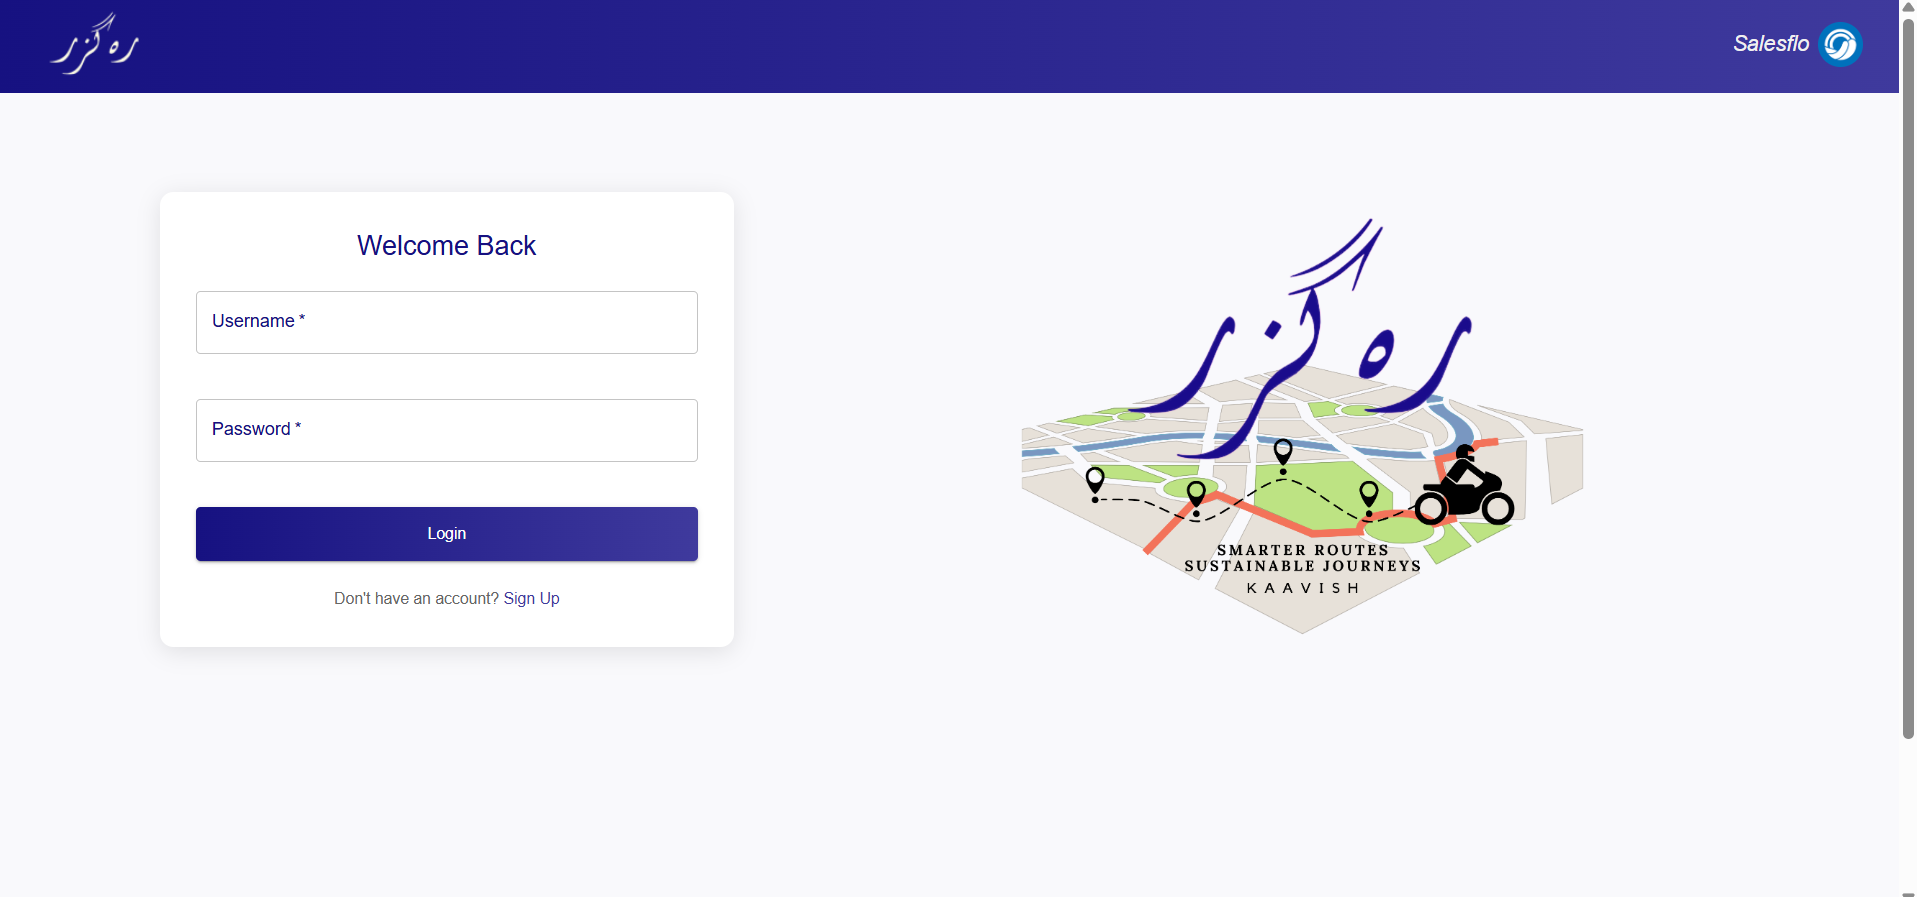
\includegraphics[width=1\textwidth]{images/Login.png} % Adjust width as needed
    \caption{Sign In Screen}
    \label{fig:image1}
\end{figure}
The sign-in screen is shown in Figure~\ref{fig:image1}, letting the user enter their email and password. They also have the option to access the sign up screen using the hyperlink in the image called "Sign up". 

\begin{figure}[H]
    \centering
    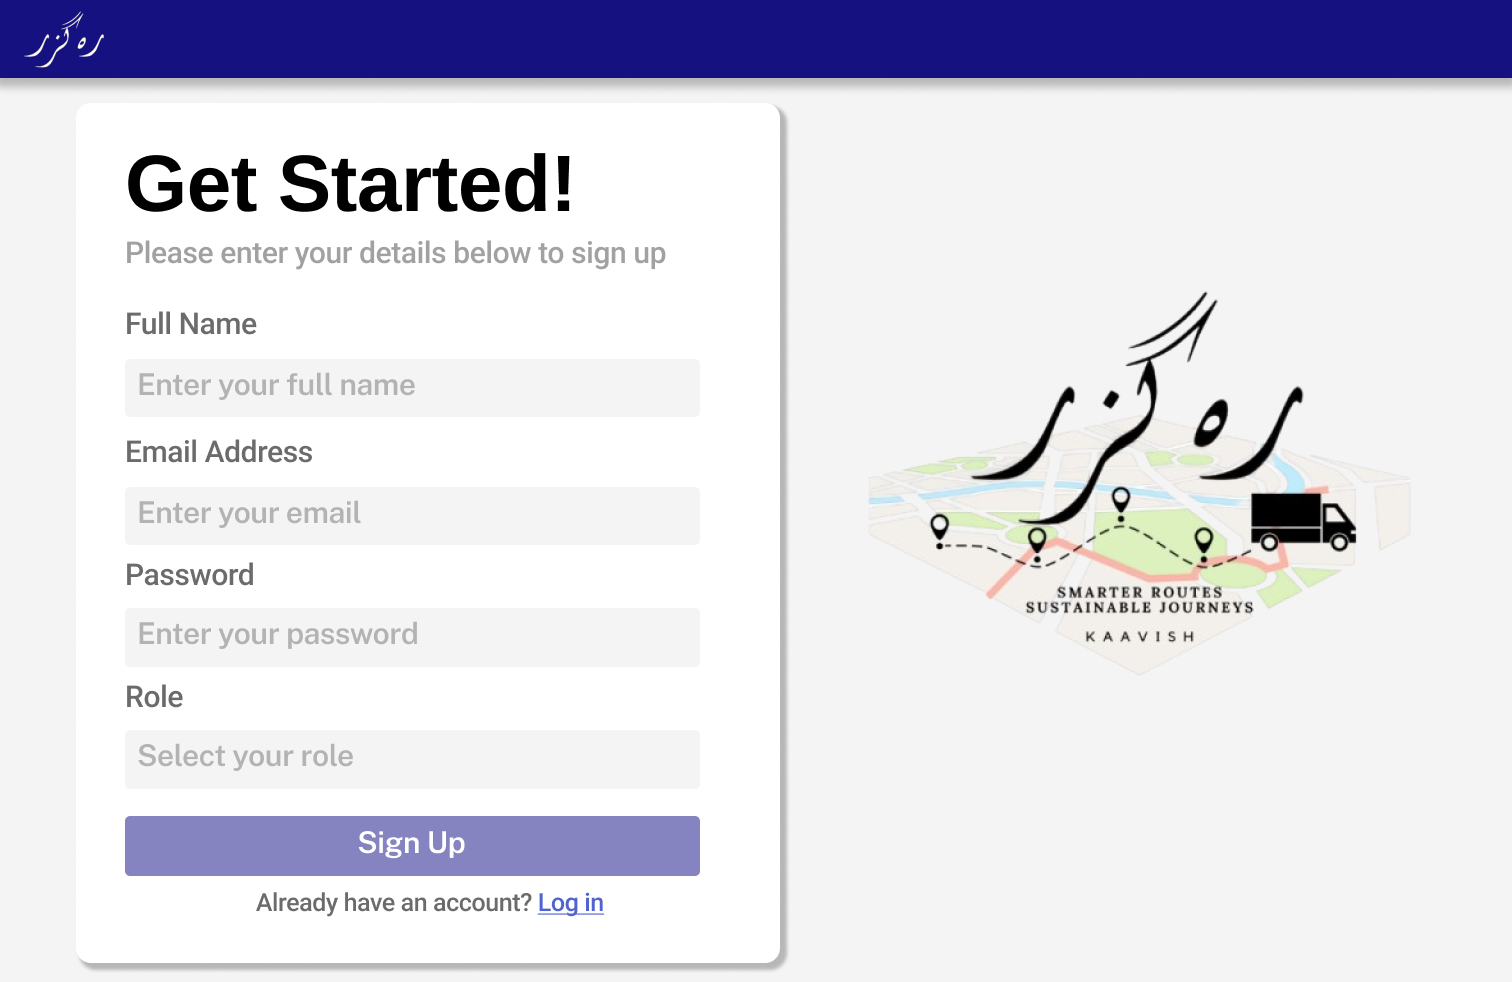
\includegraphics[width=1\textwidth]{images/Sign Up.png} % Adjust width as needed
    \caption{Sign Up Screen}
    \label{fig:image2}
\end{figure}
The sign-up screen is shown in Figure~\ref{fig:image2}, letting the user enter their full name, email and password to create an account.

\begin{figure}[H]
    \centering
    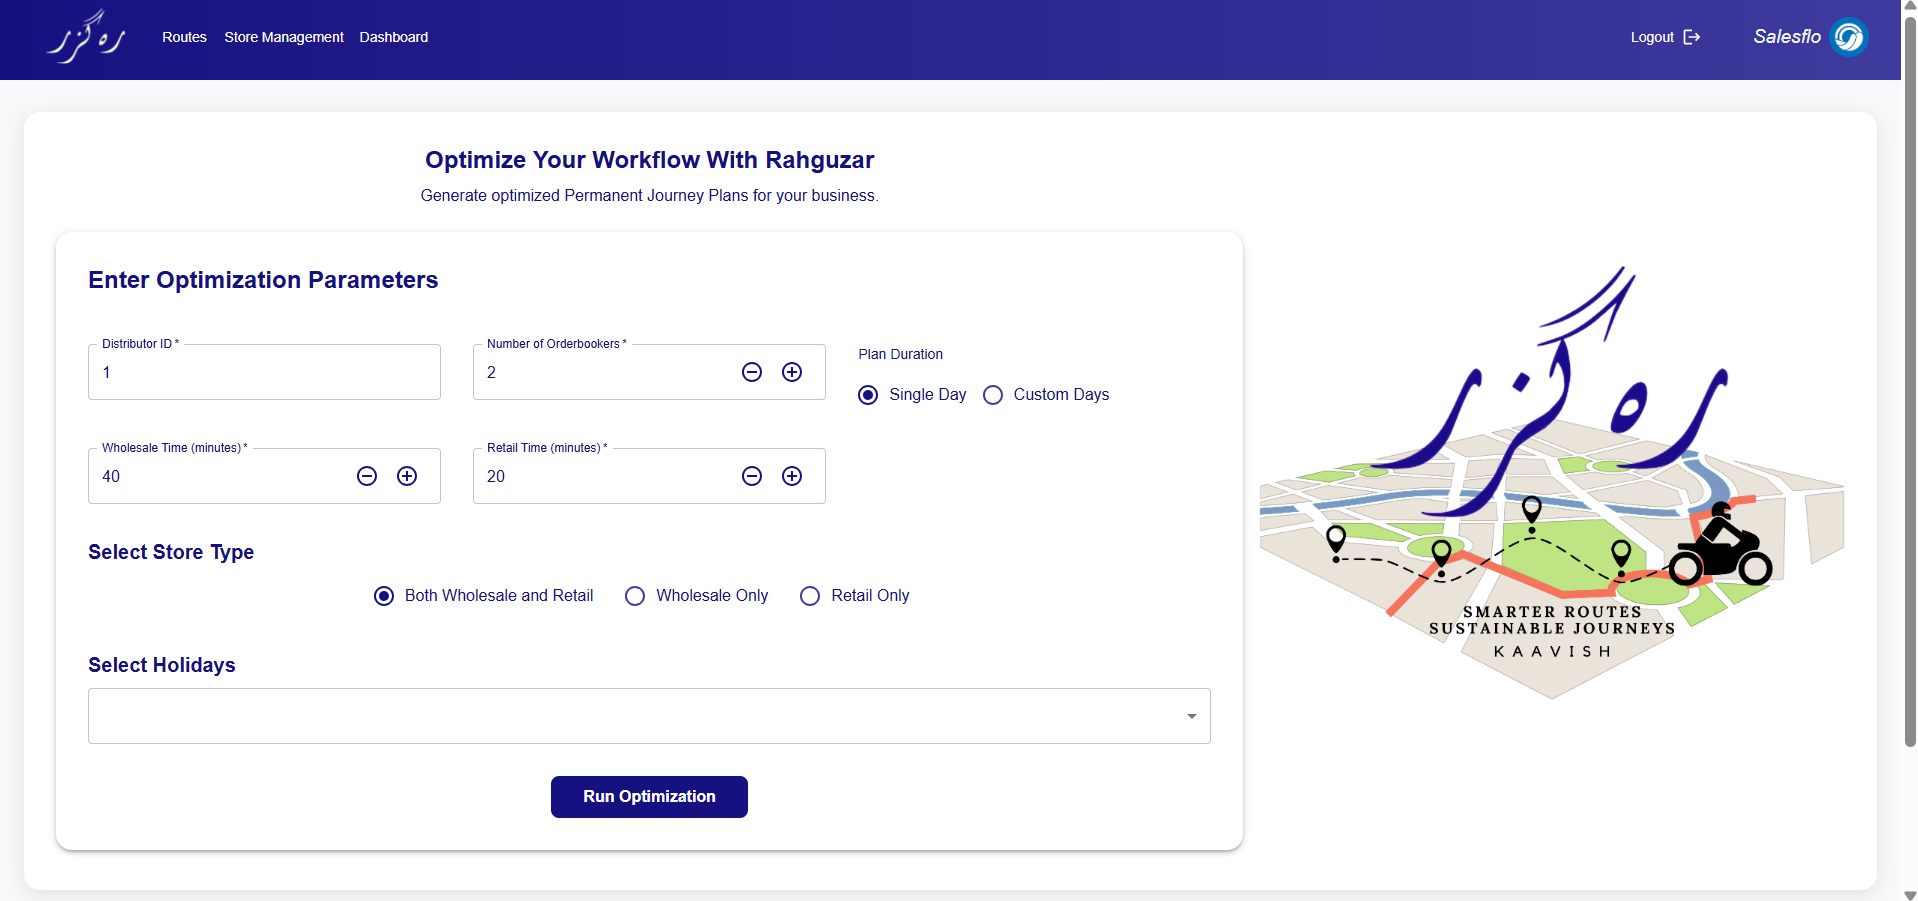
\includegraphics[width=1\textwidth]{images/Home.png} % Adjust width as needed
    \caption{Home Page}
    \label{fig:image3}
\end{figure}
The ``Home Page" screen is shown in Figure~\ref{fig:image3}, letting the user see the statistics of the day such as pending and completed orders. The user can view the upcoming recent journey and its related information such as starting and ending points, the total distance of the journey. The user will also be seeing the list of active routes and journeys that are/ will be taking place throughout the day.

\begin{figure}[H]
    \centering
    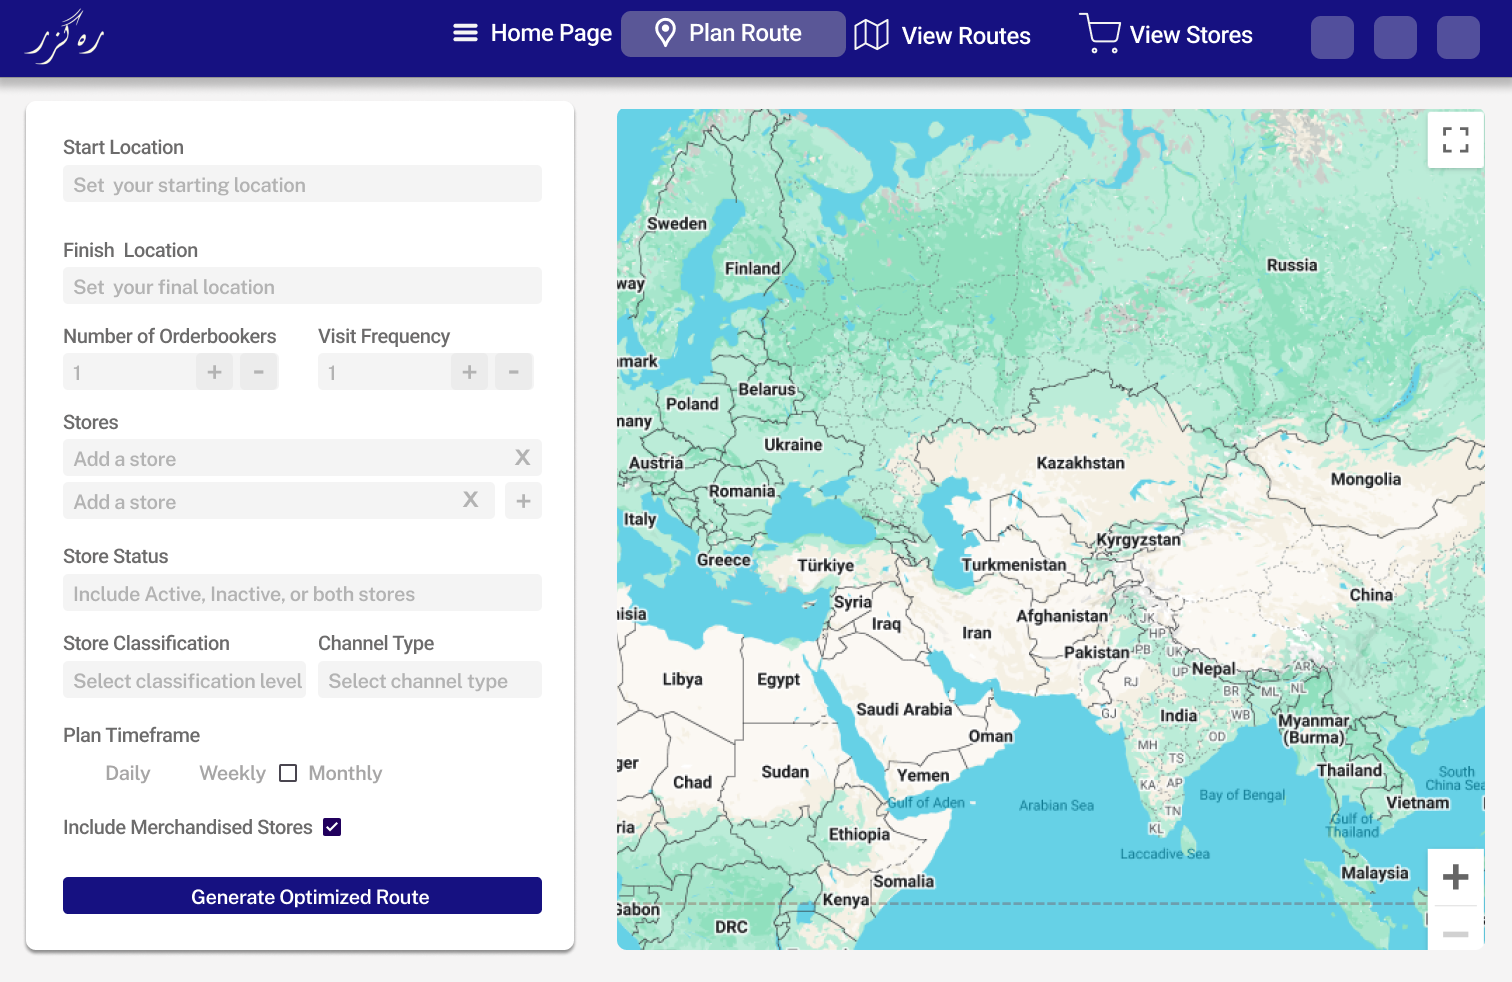
\includegraphics[width=1\textwidth]{images/Plan Route.png} % Adjust width as needed
    \caption{Plan Route Page}
    \label{fig:image4}
\end{figure}
The ``Plan Route" screen is shown in Figure~\ref{fig:image4}. In this screen, the manager will be able to create routes by setting the starting point, adding the stores to stop at, the number of orderbookres that will be involved in the journey, apply filters to stores by their classification code and choosing if they want to include only merchandised stores in the plan. Moreover, the manager can make these routes for a single day, week, or a month.

\begin{figure}[H]
    \centering
    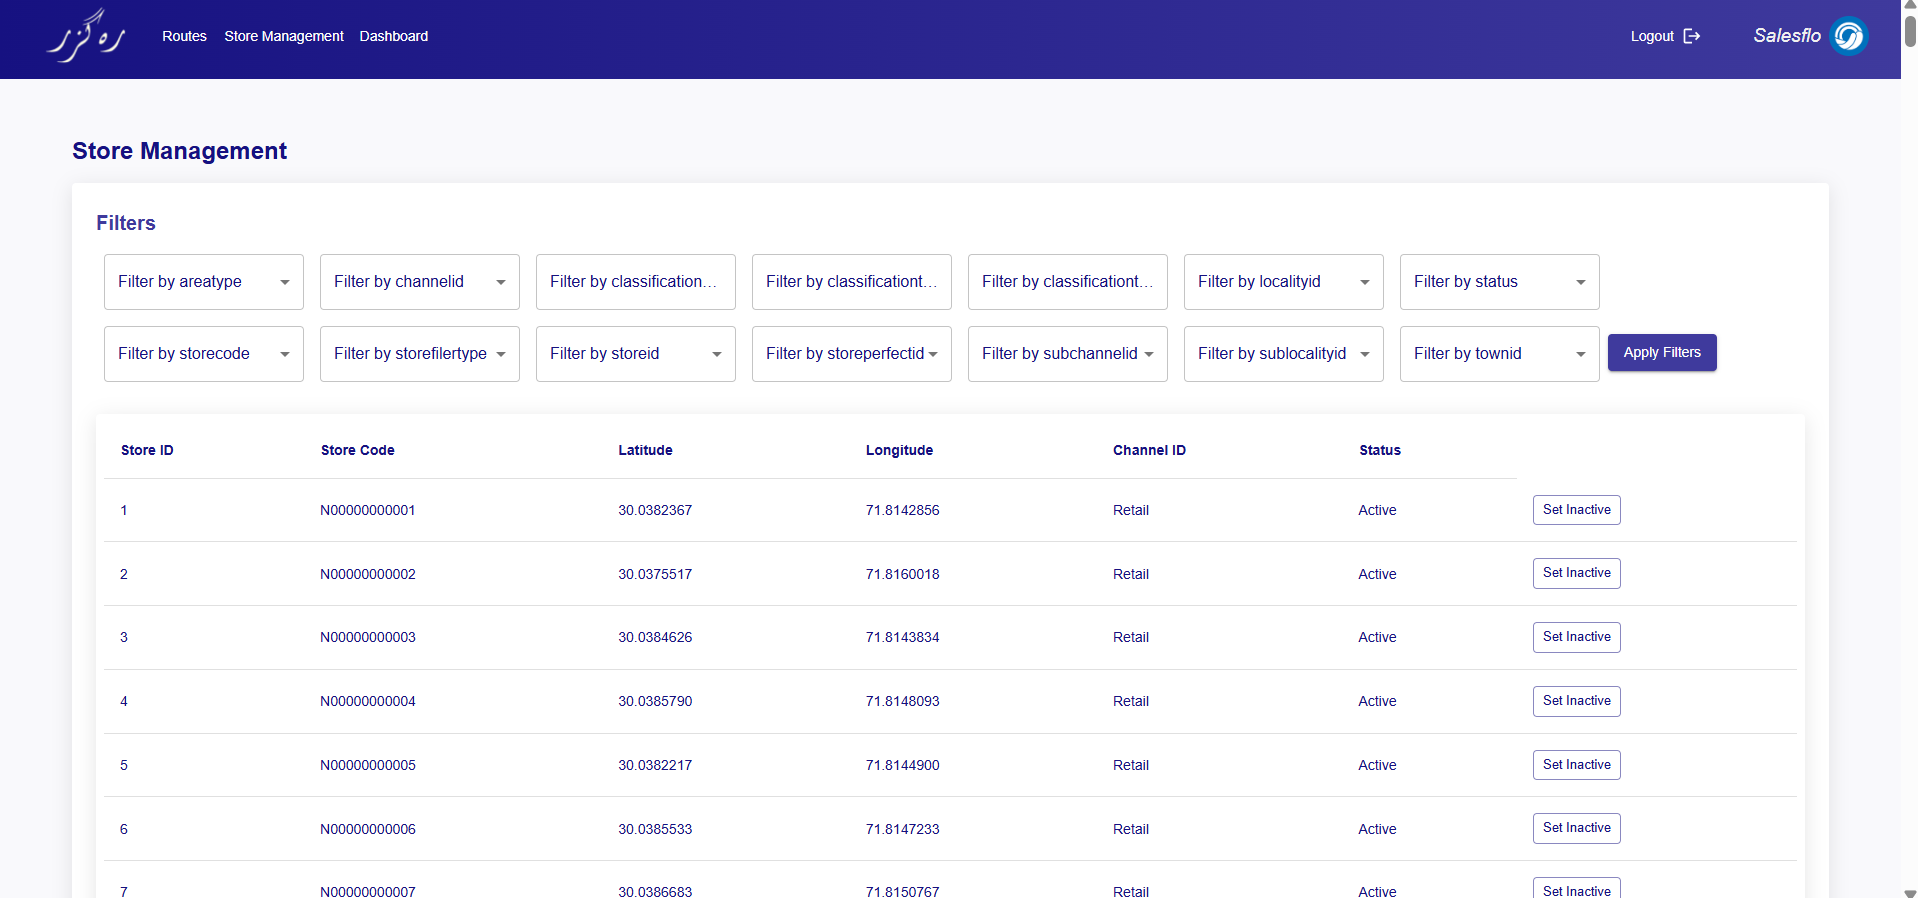
\includegraphics[width=1\textwidth]{images/View Stores.png} % Adjust width as needed
    \caption{View Stores Page}
    \label{fig:image5}
\end{figure}
The ``View Stores" screen is shown in Figure~\ref{fig:image5}. In this screen, the manager will be able to search a certain store and view its information such as its coordinates, its geographical hierarchy. They will be able to see the stores location on the map along with past orderbooker visits data. The manager has the option to view more than 1 store's information at a time.

\begin{figure}[H]
    \centering
    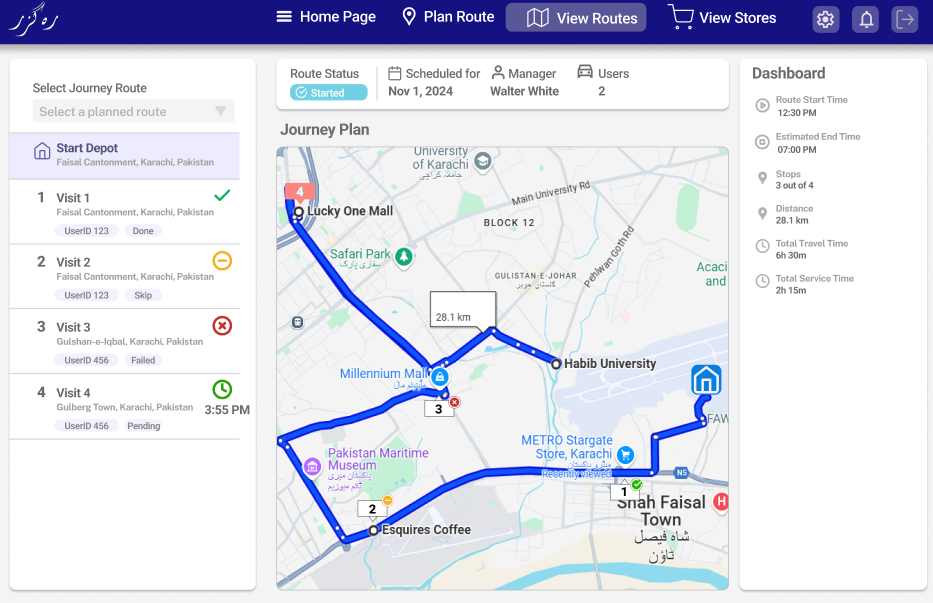
\includegraphics[width=1\textwidth]{images/View Routes.png} % Adjust width as needed
    \caption{View Routes Page}
    \label{fig:image6}
\end{figure}
The ``View Routes" screen is shown in Figure~\ref{fig:image6}. In this screen, the manager will be able to select a certain route and view its information such as the sets of locations it is comprised of, the status of the route. If a certain route has started the manager can see the status of each store location (whether it has been visited or not, the estimated time of visiting). Moreover, the manager can access the dashboard that displays route information such as the starting adn estimated end time, the total distance of the route, the distance covered by it and the number of stops involved.

\begin{figure}[H]
    \centering
    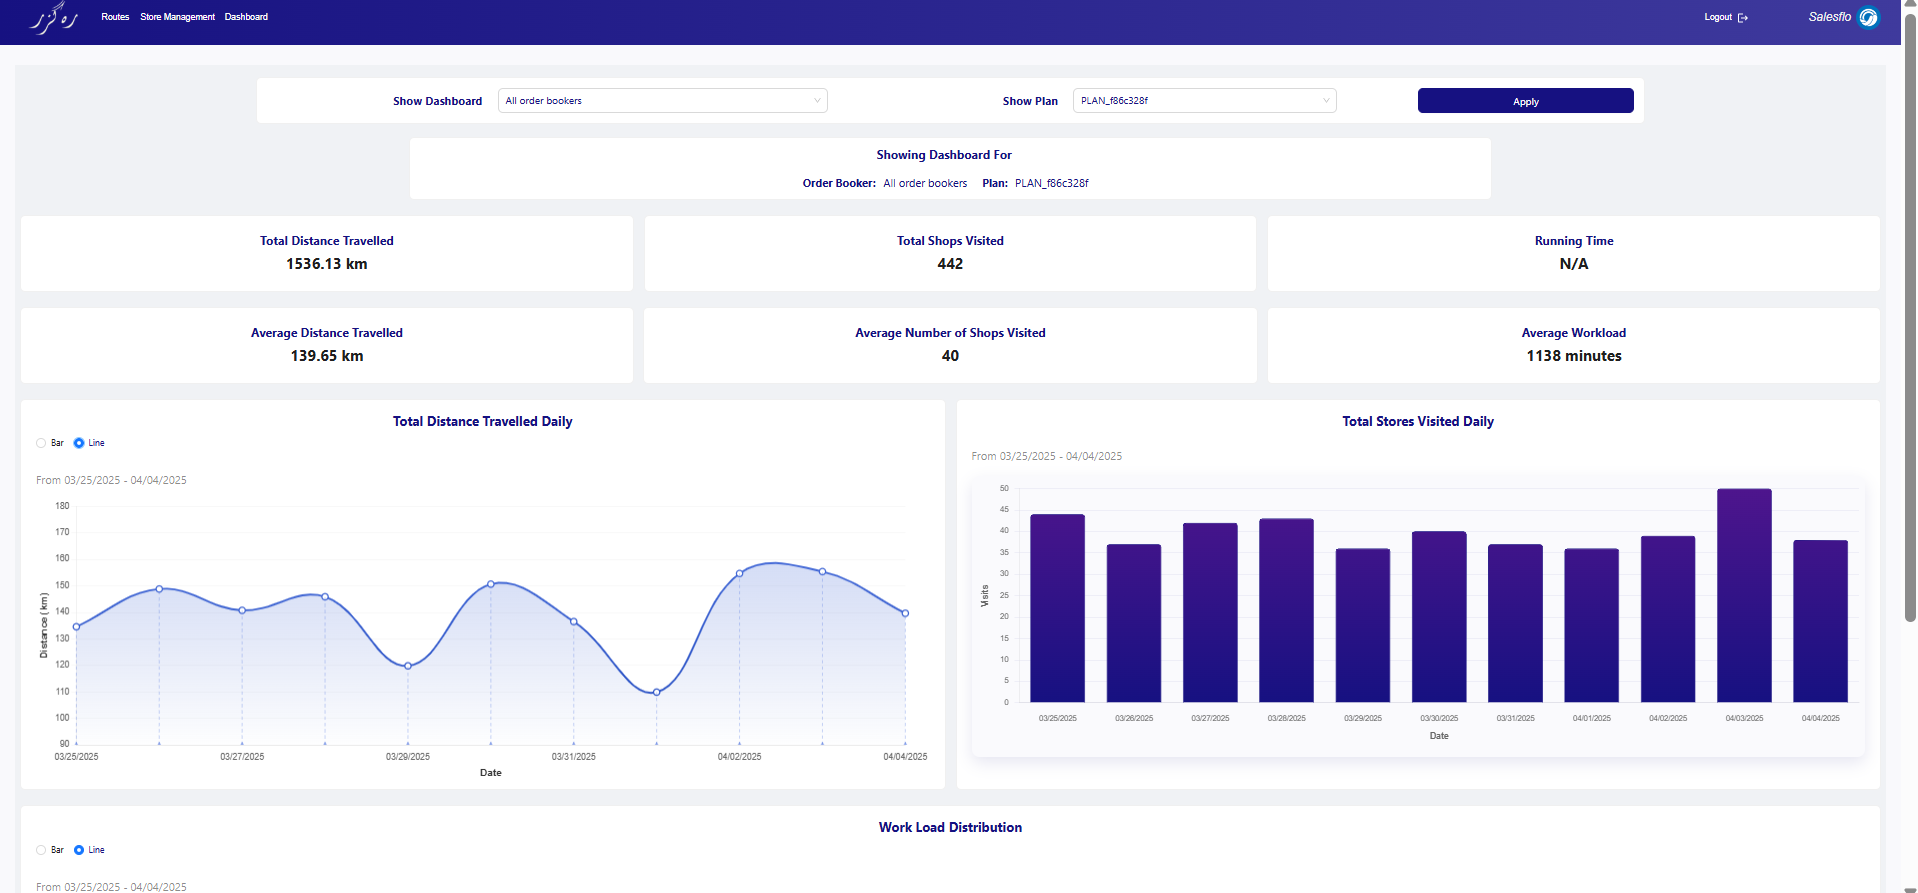
\includegraphics[width=1\textwidth]{images/Dashboard 2.png} % Adjust width as needed
    \caption{Dashboard Page}
    \label{fig:image7}
\end{figure}
The ``Dashboard" screen is shown in Figure~\ref{fig:image7}. In this screen, the manager will be able to view certain KPIs that indicate the overall performance of the routes such as Average Daily Sales per Sales Representative, Average travel time per route, and etc. 

\subsection{Application Program Interface (API)}
The API layer is the backbone of our system, enabling seamless communication between the frontend, backend, and external services. Designed to support efficient data exchange and operational scalability, this API structure ensures the system remains responsive and adaptable to business needs.

\subsubsection{REST API Endpoints}
The system is built with RESTful API endpoints that manage data transfer between components. Key endpoints include:
\begin{itemize}
    \item \textbf{Route Management Endpoints:} These endpoints facilitate route creation, configuration, and optimization. Managers can define routes, set parameters such as shift times, service times, and visit frequency, and retrieve optimized route plans tailored to specific business needs.
    \item \textbf{Visit Management Endpoints:} Used to track and manage visits by field representatives. These endpoints enable updates on visit status, start and end times, store visit durations, and compliance with predefined visit schedules.
    \item \textbf{Store Profile Endpoints:} This set of endpoints allows access to and modification of store data. Store profiles include geographic location, classification, operational hours, and specific requirements, supporting managers in executing their tasks efficiently.
\end{itemize}

\subsubsection{Authentication and Authorization}
To secure API access, the Rahguzar system employs JWT (JSON Web Tokens) for user authentication, ensuring that only authorized users can access or modify data.
\begin{itemize}
    \item \textbf{JWT Authentication:} When a user logs in, a JWT is issued and must be included with all subsequent requests. This token-based approach enhances security by verifying user identity on each API call.
\end{itemize}

\subsubsection{External Services Integration}
To support essential functionalities like mapping, the Rahguzar system integrates with external services:
\begin{itemize}
    \item \textbf{Google Maps API:} This API provides map visualization and geolocation services, enabling managers and field staff to view real-time route details. It is also used for calculating distances, travel times, and generating optimized paths between stops on a route.
\end{itemize}

\subsubsection{Route Optimization Engine}
The Route Optimization Engine is a core component of Rahguzar, leveraging advanced algorithms to generate efficient routes.
\begin{itemize}
    \item \textbf{Python + OR-Tools Integration:} Built on Python with OR-Tools, this engine generates optimized routes by balancing factors such as total travel time, number of stops, and time spent at each store. This feature is essential for ensuring that routes are aligned with operational goals while maximizing efficiency.
    \item \textbf{Geospatial Services (Geopy):} Geopy is used for geocoding services and calculating geospatial data, helping to accurately map store locations and account for distances between various stops. This service plays a key role in generating precise, reliable routes for field operations.
\end{itemize}

\subsubsection{Data Synchronization}
The system employs MongoDB as the primary data store, providing robust data storage and synchronization capabilities.
\begin{itemize}
    \item \textbf{Database Sync with MongoDB:} All route data, store profiles, and visit records are stored in MongoDB, ensuring persistent storage of essential information. MongoDB’s flexibility supports the diverse data needs of the Rahguzar system, from route optimization to visit management.
    \item \textbf{Data Update Mechanisms:} The system includes mechanisms to synchronize data across different modules and handle real-time updates, especially for managers and field staff working offline. This ensures data integrity and consistency, even in dynamic environments. To ensure scalability and high availability, MongoDB and related services are hosted on a cloud platform such as AWS, enabling the system to handle larger datasets and user traffic efficiently as the application scales.
\end{itemize}

\subsubsection{Data Monitoring}
To enable effective monitoring, the API supports data updates and performance tracking:
\begin{itemize}
    \item \textbf{Performance Analytics:} API endpoints allow managers to monitor route efficiency through Key Performance Indicators (KPIs), such as average travel time, visit completion rates, and operational metrics. This feature facilitates continuous improvement of route plans and decision-making based on real data, backed by scalable cloud infrastructure for robust data processing and analytics.
\end{itemize}


\subsection{Hardware/Communication Interfaces}
Our System relies on specific hardware and communication protocols to ensure seamless operation and efficient data management.

\subsubsection{Client-Side Hardware Requirements}
Manager Workstations: Managers access the system through web browsers on desktops or laptops for route planning and monitoring. Recommended specifications include:
\begin{itemize}
    \item \textbf{Processor:} Dual-core or higher.
    \item \textbf{RAM:} 4GB minimum.
    \item \textbf{Internet Connection:} Stable broadband with at least 5 Mbps for real-time data processing.
    \item \textbf{Browser Compatibility:} Supports modern web browsers like Chrome, Firefox, and Edge.
\end{itemize}

\subsubsection{Server-Side Infrastructure}
Cloud-Based Servers: The backend system, hosted on a cloud platform such as AWS, provides scalability, availability, and fault tolerance. Specifications include:
\begin{itemize}
    \item \textbf{Processor:} Multi-core virtual CPUs (e.g., AWS EC2).
    \item \textbf{Memory:} 4GB or more, scalable as required.
    \item \textbf{Storage:} SSD-based storage for rapid access to route, store, and visit data.
    \item \textbf{Network Configuration:} Configured for secure HTTPS communication to maintain data integrity and privacy.
\end{itemize}

\subsubsection{Communication Interfaces}
\begin{itemize}
    \item \textbf{Internet Connection:} All interactions between the frontend and backend rely on a stable internet connection for data synchronization and API requests.
\newpage
    \item \textbf{Data Communication Protocols:}
    \begin{itemize}
        \item \textbf{HTTPS:} Secure communication between frontend, backend, and external services like Google Maps API.
        \item \textbf{API Calls:} RESTful API requests enable data transfer for route management, visit updates, and user authentication.
    \end{itemize}
\end{itemize}

\subsubsection{External Services Communication}
Google Maps API: Used for map visualization, geolocation, and distance calculation, requiring internet connectivity for location-based data.


\section{Use Cases}
\begin{itemize}
    \item \textbf{User Authentication and Access Control}
    \begin{itemize}
        \item \textbf{Description:} Ensure secure access to the system for both managers and field staff.
        \item \textbf{Actions:}
        \begin{itemize}
            \item As a manager, I want to log in securely to access my dashboard and manage routes.
            \item As the system, I need to authenticate users to ensure only authorized managers and field staff access the application.
        \end{itemize}
    \end{itemize}
    
    \item \textbf{Route Creation, Configuration, and Optimization}
    \begin{itemize}
        \item \textbf{Description:} Enable the creation of optimized routes based on configurable parameters.
        \item \textbf{Actions:}
        \begin{itemize}
            \item As a manager, I want to create a new optimized route for my field team, configuring parameters like shift timings and visit frequency to align with operational requirements.
            \item As the system, I need to generate optimized routes using parameters such as shift times, visit frequencies, and priorities, ensuring efficient route suggestions for managers.
        \end{itemize}
    \end{itemize}
    
    \item \textbf{Dynamic Rerouting and Manual Overrides}
    \begin{itemize}
        \item \textbf{Description:} Allow for real-time adjustments to routes, either dynamically by the system or manually by the manager.
        \item \textbf{Actions:}
        \begin{itemize}
            \item As a manager, I want to make manual adjustments to routes to adapt to urgent needs or unexpected changes.
            \item As a manager, I want the system to dynamically reroute based on parameter changes after the route is generated.
            \item As the system, I need to recalculate routes dynamically if the manager makes changes to parameters, ensuring updated routes without disrupting existing operations.
        \end{itemize}
    \end{itemize}
    
    \item \textbf{Route Sharing and Export}
    \begin{itemize}
        \item \textbf{Description:} Facilitate the sharing of finalized routes with field staff.
        \item \textbf{Actions:}
        \begin{itemize}
            \item As a manager, I want to export and share finalized routes with field staff so they have clear guidance on their daily tasks and destinations.
            \item As the system, I need to support data export so that managers can download route plans and reports for offline access if needed.
        \end{itemize}
    \end{itemize}
    
    \item \textbf{Plan Generation (Weekly/Monthly)}
    \begin{itemize}
        \item \textbf{Description:} Generate long-term journey plans based on store visit requirements.
        \item \textbf{Actions:}
        \begin{itemize}
            \item As a manager, I want the ability to generate weekly or monthly journey plans, providing my team with a consistent schedule for store visits.
            \item As the system, I need to automatically generate journey plans for weekly and monthly schedules based on specified visit frequencies.
        \end{itemize}
    \end{itemize}
    
    \item \textbf{Store Profile Integration and Viewing}
    \begin{itemize}
        \item \textbf{Description:} Provide access to detailed store profiles to aid in route planning.
        \item \textbf{Actions:}
        \begin{itemize}
            \item As a manager, I want to view detailed store profiles, including location and sales channel, to prioritize visits and plan routes effectively.
            \item As the system, I need to integrate and maintain comprehensive store profiles, making it easier for managers to access relevant data during route planning.
        \end{itemize}
    \end{itemize}
    
    \item \textbf{Interactive Map Visualization}
    \begin{itemize}
        \item \textbf{Description:} Enable map-based visualization of routes and store locations.
        \item \textbf{Actions:}
        \begin{itemize}
            \item As a manager, I want to see routes on an interactive map, allowing me to visualize store locations and make adjustments as needed.
            \item As the system, I need to display routes and navigation data on an interactive map interface for both managers and field staff.
        \end{itemize}
    \end{itemize}
    
    \item \textbf{Performance Tracking and KPI Monitoring}
    \begin{itemize}
        \item \textbf{Description:} Track and analyse performance metrics to evaluate route effectiveness.
        \item \textbf{Actions:}
        \begin{itemize}
            \item As a manager, I want to track KPIs like travel time and visit completion rates to assess route performance and make improvements.
            \item As the system, I need to automate KPI tracking (e.g., average travel time, visit completion) to provide ongoing insights without requiring manual input from managers.
        \end{itemize}
    \end{itemize}
    
    \item \textbf{System Data Synchronization}
    \begin{itemize}
        \item \textbf{Description:} Sync store and route data to ensure accurate and up-to-date information.
        \item \textbf{Actions:}
        \begin{itemize}
            \item As a manager, I want the system to view store information and route statuses, giving me reliable data for decision-making.
            \item As the system, I need to synchronize with external databases to maintain current and accurate store and route data for all users.
        \end{itemize}
    \end{itemize}
    
    \item \textbf{Store Visit Recording and Analysis}
    \begin{itemize}
        \item \textbf{Description:} Record visit details and enable analysis of visit data for operational insights.
        \item \textbf{Actions:}
        \begin{itemize}
            \item As a manager, I want each store visit’s details recorded, allowing me to analyse time spent and identify areas for improvement.
            \item As the system, I need to log each store visit's start time, end time, and duration, providing accurate records for analysis and performance tracking.
        \end{itemize}
    \end{itemize}
    
    \item \textbf{Pilot Testing and Validation}
    \begin{itemize}
        \item \textbf{Description:} Conduct pilot tests to validate system effectiveness in real-world scenarios.
        \item \textbf{Actions:}
        \begin{itemize}
            \item As a manager, I want to test the system in a pilot environment to evaluate its performance and impact before full deployment.
            \item As the system, I need to support pilot testing by recording metrics during live tests, allowing managers to assess effectiveness and identify areas for improvement.
        \end{itemize}
    \end{itemize}
    
\end{itemize}

\begin{center}
    \begin{figure}[H]
        \centering
        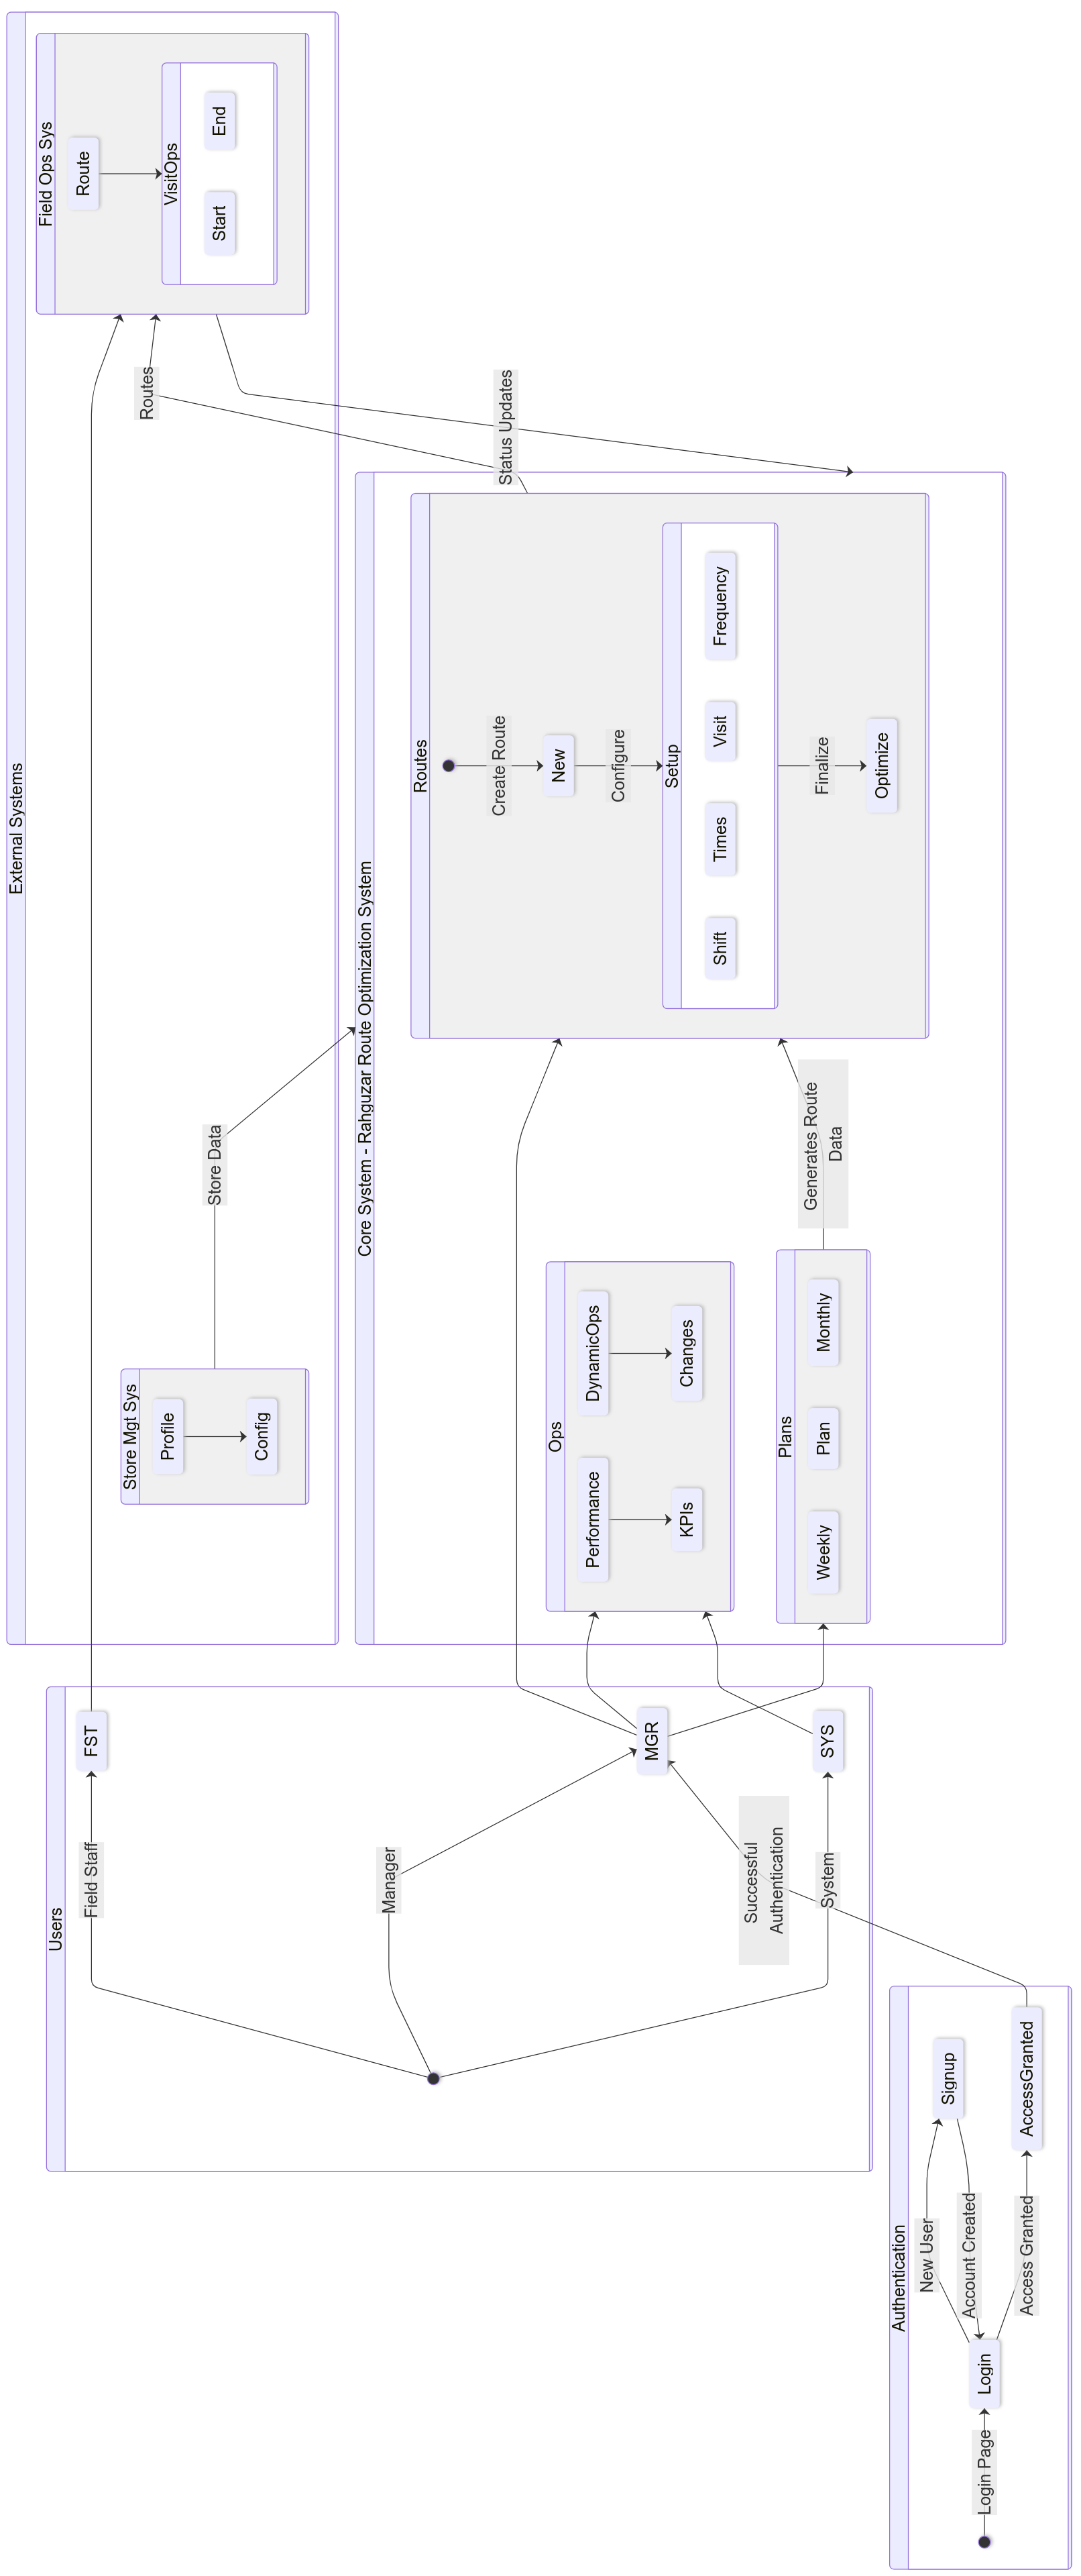
\includegraphics[width=0.6\textwidth]{images/Rahguzar - Use Case - HighLevel (1).png} 
        \caption{Rahguzar's High-Level Use Case Diagram for the Entire System}
\href{https://tinyurl.com/USECASEDIAG}{(Click here to view a high-quality version of this image)}
    \end{figure}

    \begin{figure}[H]
        \centering
        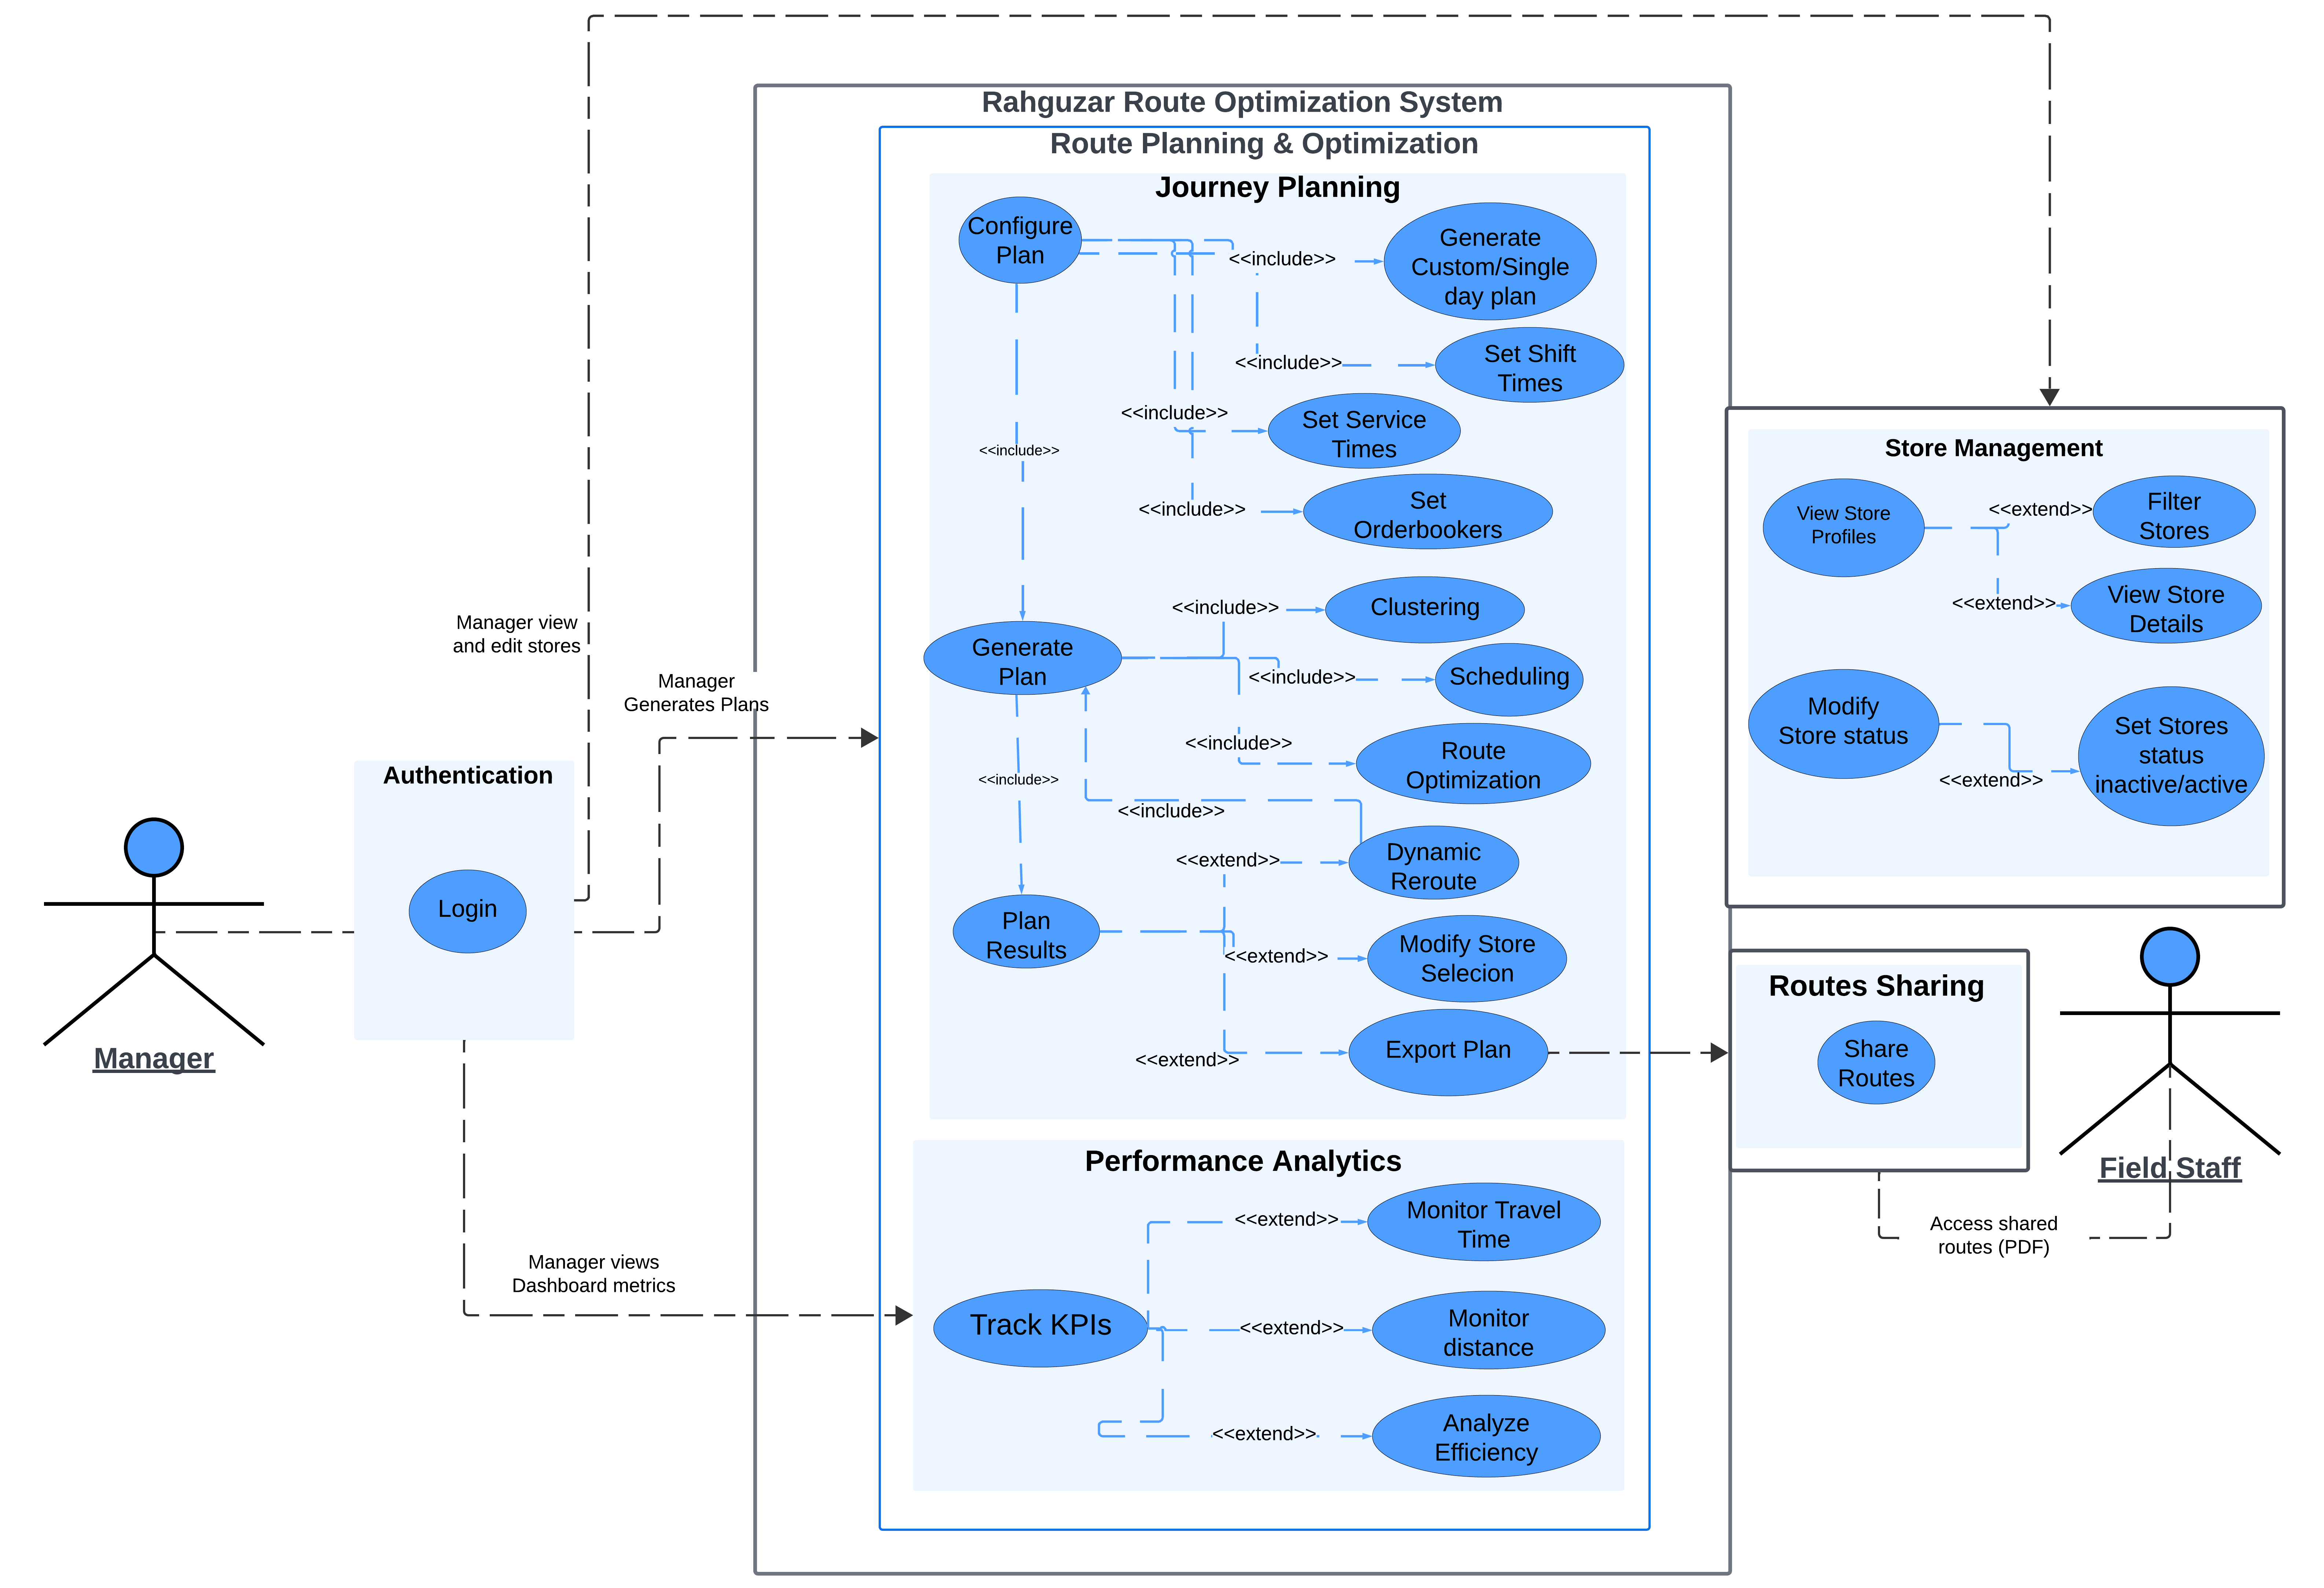
\includegraphics[width=0.98\textwidth]{images/Rahguzar - Use Case - Core System.png} 
        \caption{Rahguzar's Core System Use Case Diagram within the Main System}
    \end{figure}
\end{center}

\section{Datasets}
% This section describes the specific dataset(s) used to build our system. An appropriate snapshot of the dataset(s) is also included. Futher details, when needed, are presented in the appendix.
This section outlines the primary datasets that will support Rahguzar’s intelligent route planning and scheduling functionalities. These datasets provide crucial information on stores, visits, journey plans, and operational factors essential for optimized route generation. As per the NDA with SalesFlo, we are not permitted to share or disclose the data provided to us. Further data and details are awaited from SalesFlo, and this section reflects the information we currently have.

\subsection*{Overview of Required Datasets}

\begin{enumerate}

\item \textbf{Store Universe} \\
This dataset provides foundational information on each store, including location, operational status, and distributor associations. Key fields include:
    \begin{itemize}
        \item \textbf{storecode:} Unique identifier for each store.
        \item \textbf{storestatus:} Operational status (active or inactive).
        \item \textbf{latitude and longitude:} Geographic coordinates.
        \item \textbf{distributorcode:} Code for the distributor linked to the store.
        \item \textbf{pjpcode:} Code for the Permanent Journey Plan (PJP) associated with the store.
    \end{itemize}
This dataset is essential for determining which stores to include in routes based on location and operational status.

\item \textbf{Store Hierarchy} \\
This dataset offers classification and hierarchical details, allowing route customization based on store attributes such as region or sales channel. Key fields include:
    \begin{itemize}
        \item \textbf{storecode:} Identifier for each store.
        \item \textbf{areatype, townid, localityid:} Geographical identifiers.
        \item \textbf{channeltypeid and channelid:} Sales channel identifiers (e.g., retail, wholesale).
        \item \textbf{storeclassificationIDs: } These classification IDs will be used to further distinguish between certain store categories.
    \end{itemize}
This data enables Rahguzar to organize routes by region and sales channel, optimizing for specific geographic and operational criteria.

\item \textbf{Visits} \\
The Visits dataset records historical visit information for each store, including time spent, visit order, and outcomes. Key fields include:
    \begin{itemize}
        \item \textbf{visitid:} Unique identifier for each visit.
        \item \textbf{pjpcode:} Journey plan code associated with the visit.
        \item \textbf{visitdate, visitstarttime, visitendtime:} Time data for analyzing visit durations.
        \item \textbf{visitspenttimeinseconds:} Total time spent at the store during the visit.
        \item \textbf{orderstatus:} Status of any order placed during the visit.
        \item \textbf{visiststatus: } Status determining if a visit has been completed or not.
        \item \textbf{syncdown, syncup, syncdowndatetime: } These fields track the synchronization status and timing of visit records: syncdown shows if data was downloaded to the device, syncup if it was uploaded to the server, and syncdowndatetime logs the last download timestamp.
    \end{itemize}
This dataset supports route optimization by providing insights into visit frequency and duration, refining future scheduling.

\end{enumerate}

\subsection*{Additional Datasets Needed}

To enhance Rahguzar's functionality, the following additional datasets may be required:

\begin{enumerate}

\item \textbf{Order Booker Shifts Dataset} \\
This dataset contains information on the availability and shifts of order bookers. Key fields include:
    \begin{itemize}
        \item \textbf{bookerid:} Unique identifier for each order booker.
        \item \textbf{shiftstarttime and shiftendtime:} Start and end times of each shift.
        \item \textbf{availabilitystatus:} Indicates whether the booker is available or unavailable.
    \end{itemize}
This dataset is essential for scheduling routes within the working hours of each order booker, optimizing route generation according to workforce availability.

\item \textbf{Geographic Data} \\
Geographic and road network data provide detailed map and routing information, potentially sourced via the Google Maps API or GIS data services. Key components include:
    \begin{itemize}
        \item \textbf{roadnetwork:} Map of roads, including distances and travel times.
        \item \textbf{trafficpatterns:} Historical traffic data for congestion analysis.
        \item \textbf{geofencingdata:} Predefined boundaries for specific zones, regions, or territories.
    \end{itemize}
This dataset enables precise route calculations, factoring in real-time or historical traffic conditions to minimize travel time.

\item \textbf{Store Activity Requirements} \\
This dataset details the specific activities and time requirements for each store visit, allowing Rahguzar to optimize for different tasks performed at each store. Key fields include:
    \begin{itemize}
        \item \textbf{storecode:} Identifier for each store.
        \item \textbf{activitytype:} Type of activity required (e.g., stock check, merchandising).
        \item \textbf{estimatedtime:} Average time required to complete each activity.
    \end{itemize}
This dataset supports the system’s ability to tailor visit durations based on store requirements, leading to more accurate time estimates for each route.
\end{enumerate}

\subsection*{Data Utilization in Rahguzar}

Together, these datasets will support Rahguzar’s core functionalities, including:
\begin{itemize}
    \item \textbf{Efficient Route Planning:} Leveraging store locations, operational statuses, and road networks for optimal routing.
    \item \textbf{Dynamic Scheduling:} Using order booker shifts and activity requirements to generate flexible schedules aligned with store needs and workforce availability.
    \item \textbf{Traffic and Geographic Optimization:} Utilizing geographic data to plan routes that avoid congestion and optimize for specific zones or territories.
    \item \textbf{Geographical Filtering:} Geographical and channel-based categorization from the Store Hierarchy dataset will help managers plan routes tailored to specific regions and sales priorities.
    \item \textbf{Route Efficiency Analysis:} The Visits dataset will provide insights into average visit durations and travel times, which will inform the route optimization algorithm and support KPI tracking for system performance.
\end{itemize}

Further details and data will be incorporated as they become available from SalesFlo.

\section{System Diagram}
\begin{center}
        \begin{figure}[H]
        \centering
        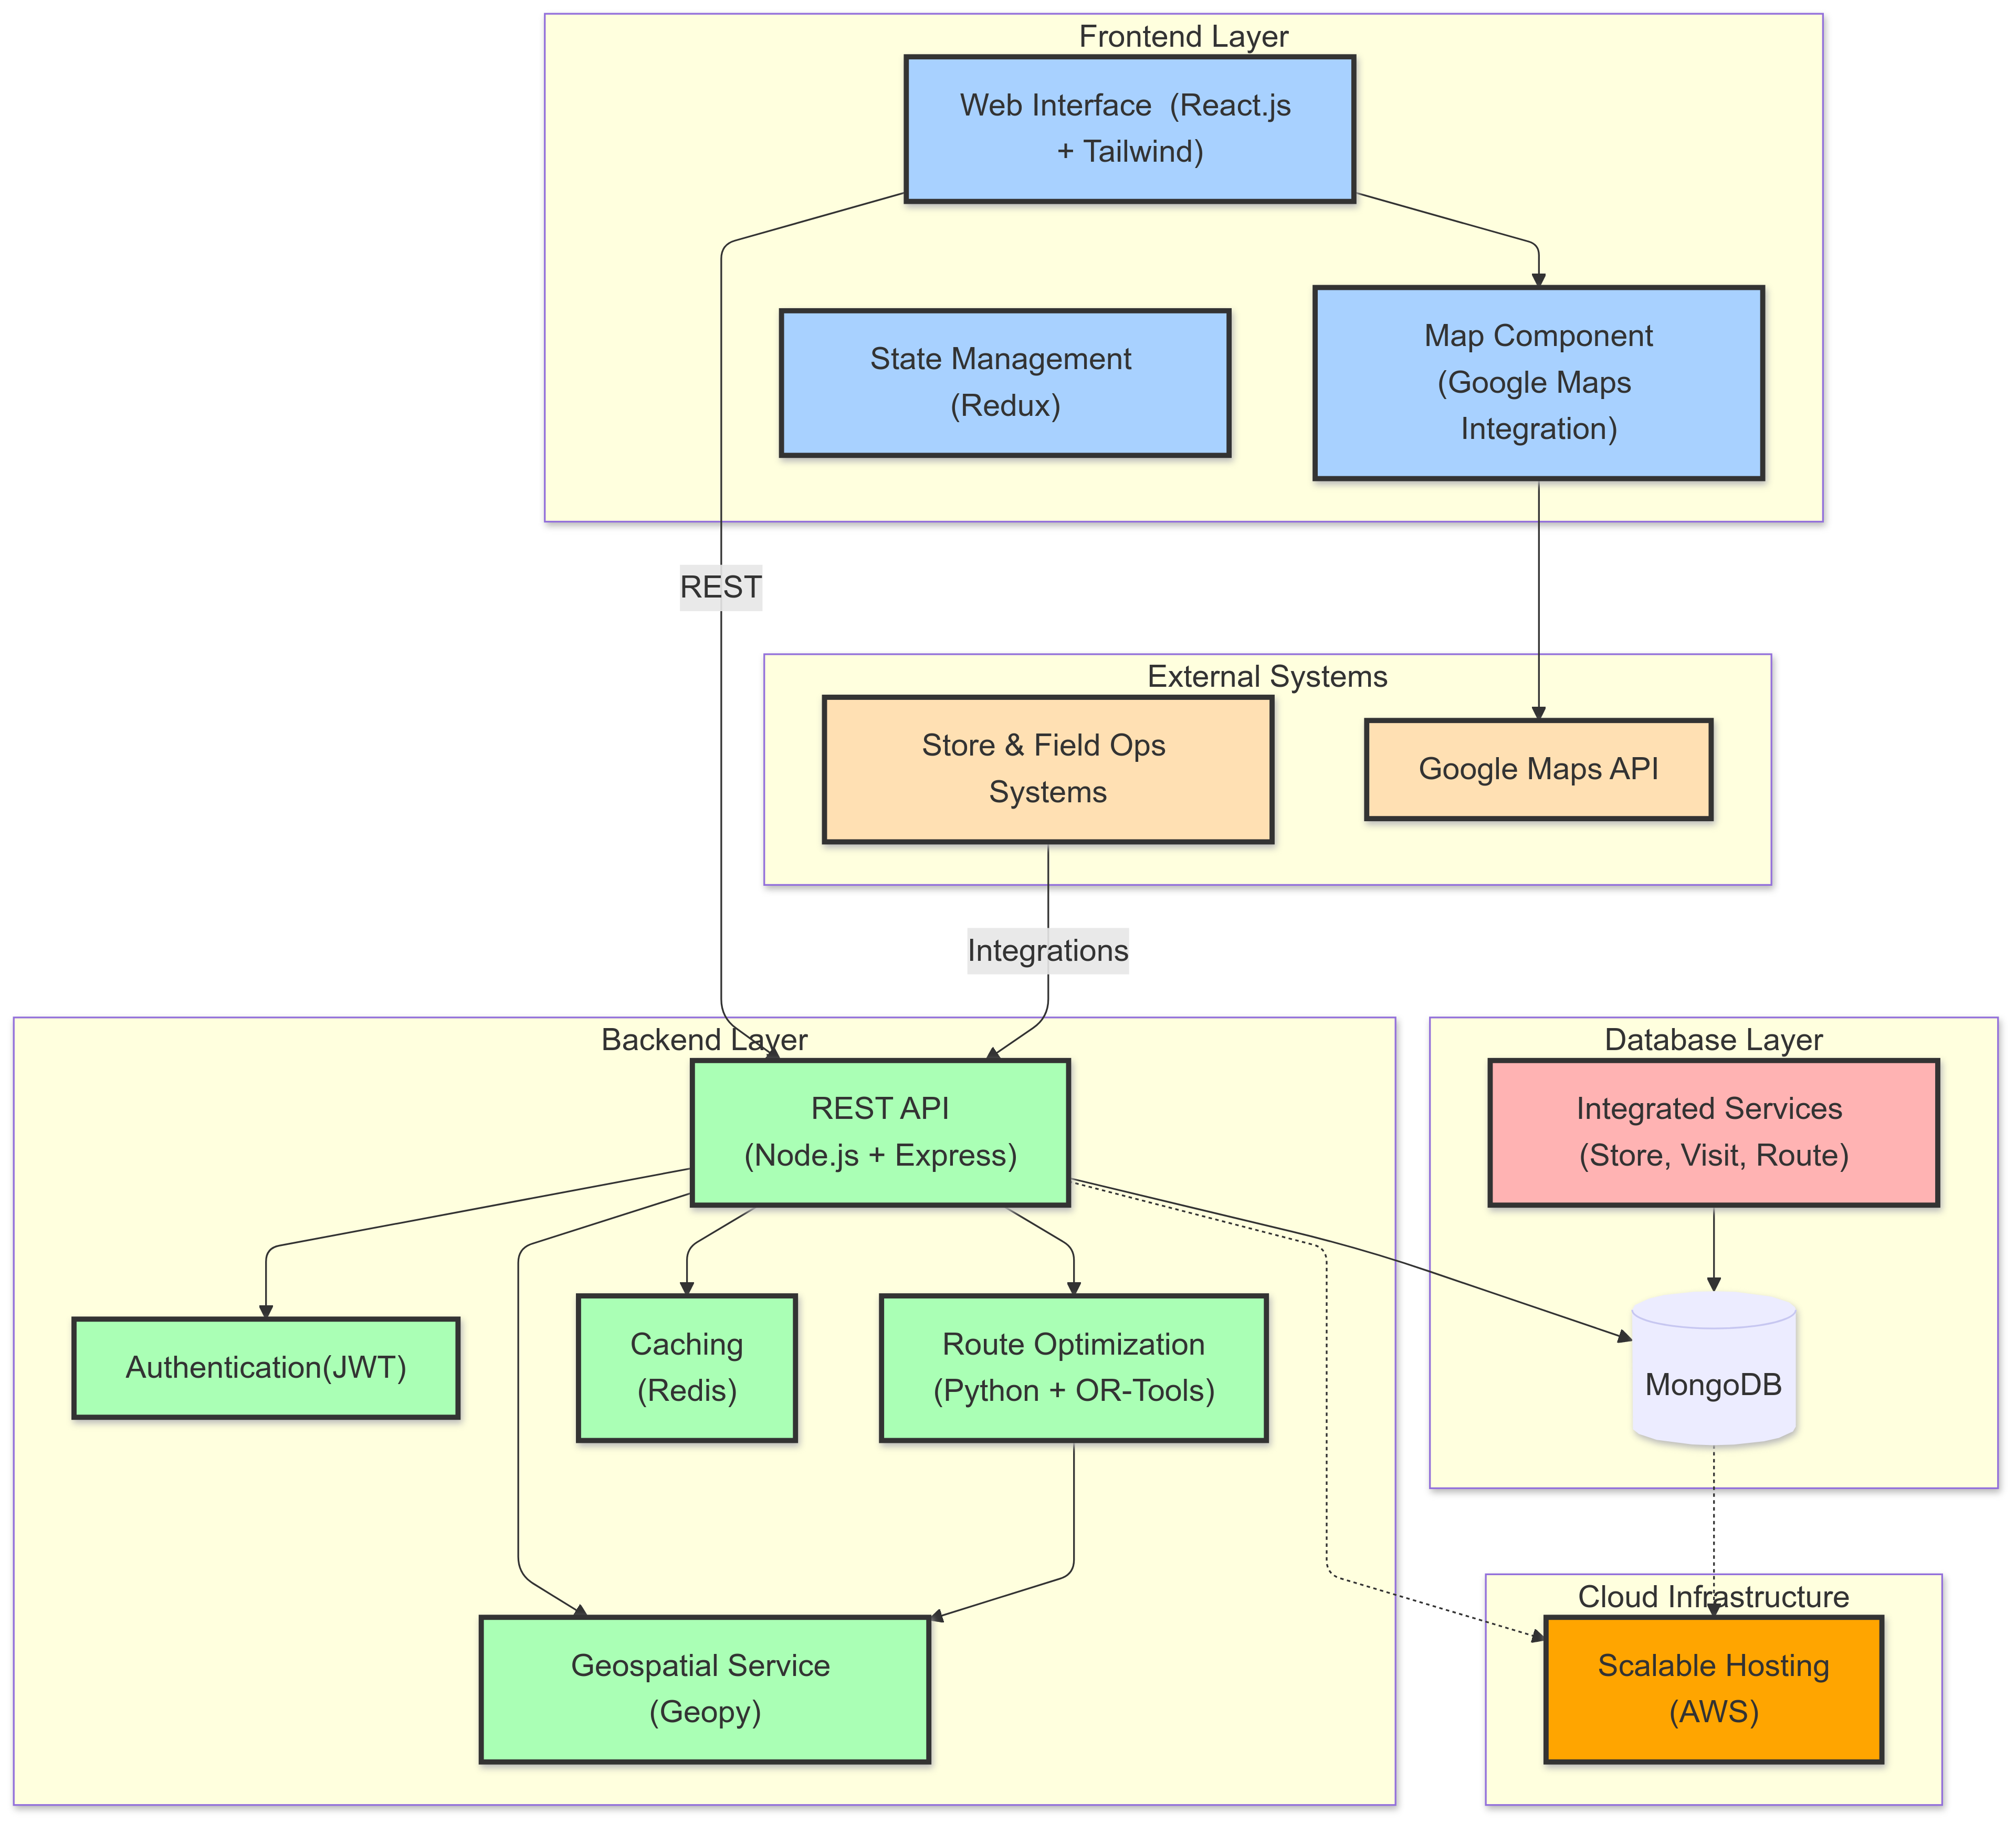
\includegraphics[width=\textwidth]{images/Rahguzar - High Level System Diagram.png} 
        \caption{Rahguzar's System Architecture Diagram}
    \end{figure}
\end{center}